\documentclass[aspectratio=43]{beamer}
\usepackage[latin1]{inputenc}
\usepackage{amsmath}
\usepackage{amsfonts}
\usepackage{amssymb}
\usepackage{makeidx}
\usepackage{graphicx}
\usepackage{array}

% Customization
\mode<presentation>{
\usetheme{CambridgeUS}
\usecolortheme{dolphin}
\setbeamertemplate{navigation symbols}{}
}

%\setbeamertemplate{footline}[frame number]

%TikZ diagrams
\usepackage{tikz}
\usetikzlibrary{patterns}
\usetikzlibrary{arrows,shapes}
\usetikzlibrary{shapes.multipart}
\usetikzlibrary{trees}
\usetikzlibrary{shapes.geometric}
\usetikzlibrary{matrix,arrows}
\usetikzlibrary{positioning}
\usetikzlibrary{calc,through}
\usetikzlibrary{decorations.pathreplacing}
\usepackage{pgffor}

% Define colors
\definecolor{darkgreen}{rgb}{0.0, 0.5, 0.13}
\definecolor{darkblue}{rgb}{0.0, 0.0, 0.55}
\definecolor{darkred}{rgb}{0.55, 0.0, 0.0}

% For using TikZ
\usetikzlibrary{decorations.pathmorphing}
\usetikzlibrary{decorations.markings}
\tikzset{
	vector/.style={decorate, decoration={snake,amplitude=3pt}, draw},
	gluon/.style={decorate, decoration={coil,amplitude=2.5pt},draw},
	provector/.style={decorate, decoration={snake,amplitude=2.5pt}, draw},
	antivector/.style={decorate, decoration={snake,amplitude=-2.5pt}, draw},
	fermion/.style={draw=black, postaction={decorate},
		decoration={markings,mark=at position .55 with {\arrow[draw=black,thick]{>}}}},
	fermionbar/.style={draw=black, postaction={decorate},
		decoration={markings,mark=at position .55 with {\arrow[draw=black,thick]{<}}}},
	fermionnoarrow/.style={draw=black},
	gluon/.style={decorate, draw=black,
		decoration={coil,amplitude=2.5pt, segment length=3pt}},
	gluon2/.style={decorate, draw=black,
		decoration={coil,amplitude=1.75pt, segment length=2.75pt}},
	scalar/.style={dashed,draw=black, postaction={decorate},
		decoration={markings,mark=at position .55 with {\arrow[draw=black]{>}}}},
	scalarbar/.style={dashed,draw=black, postaction={decorate},
		decoration={markings,mark=at position .55 with {\arrow[draw=black]{<}}}},
	scalarnoarrow/.style={dashed,draw=black},
	electron/.style={draw=black, postaction={decorate},
		decoration={markings,mark=at position .55 with {\arrow[draw=black]{>}}}},
	bigvector/.style={decorate, decoration={snake,amplitude=4pt}, draw},
}

% Blocks
\tikzstyle{block} = [draw, rectangle, minimum height = 3em, rounded corners, minimum width = 4em]
\tikzstyle{block2} = [draw, rectangle, minimum height = 3em, rounded corners, minimum width = 7em]
\tikzstyle{circle} = [draw, circle, radius = 1.5]
\tikzstyle{arrow} = [thick,->]
%************************************************************************************************************

% Title and author
\title[QCD and Monte Carlo]{QCD and Monte Carlo}
\author{\textbf {Jes\'us Urtasun Elizari}}
%\institute{\textbf {University of Milan}}
\date{Milan, September 2020}

\begin{document}

% Front slide
\begin{frame}

	%\maketitle
	\vspace{1.0 cm}
	
	\center{\color{blue}Perturbative QCD and Monte Carlo event generators}
	
	\vspace{0.25 cm}
	\center{Monte Carlo course seminar - Milan, September 2020}

	\begin{figure}
		\minipage{1\textwidth}
		
\includegraphics[width = 3.0 cm]{plots/logo_unimi.png}
		\hfill
		
\includegraphics[width = 3.0 cm]{plots/logo_infn.png}
		\hfill
		
\includegraphics[width = 3.0 cm]{plots/logo_erc.png}
		\endminipage
	\end{figure}

	\vspace{1.0 cm}

\end{frame}

% Introduction
\begin{frame}

	\frametitle{Outline}
	
	\begin{enumerate}
		\item {\color{blue}Hadron collisions}
		\begin{itemize}
			\item Hadron collisions and strong interactions
			\item Renormalization group
			\item Jets and IR divergences
		\end{itemize}
		\item {\color{blue}Collinear factorization}
		\begin{itemize}
			\item Factorization theorem
			\item Kinematics of splitting
			\item Fixed Order calculations
		\end{itemize}
		\item {\color{blue}Parton showers}
		\begin{itemize}
			\item Final state radiation
			\item Initial state radiation
			\item Ordering variables (PYTHIA and HERWIG)
		\end{itemize}
	\end{enumerate}
	
\end{frame}

% Hadron collisions
\begin{frame}

\center{\color{blue}Hadron collisions}

\end{frame}

% Hadron collisions I
\begin{frame}

	\frametitle{Hadron collisions}
	\framesubtitle{QCD from $e^{+}e^{-}$ annihilation}

	\begin{figure}
		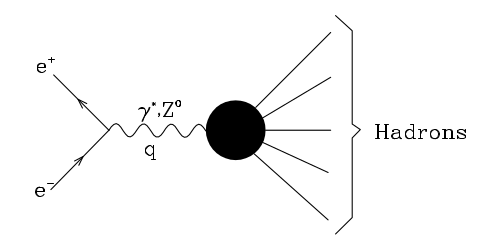
\includegraphics[width = 5 cm]{plots/ee_hadrons.png}
	\end{figure}
 
	QCD arise already from $e^{+}e^{-}$ annihilation $\rightarrow R_{0}$ ratio
	\begin{figure}
		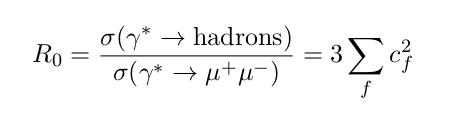
\includegraphics[width = 6 cm]{plots/eq_R0.png}
	\end{figure}

	\begin{enumerate}
		\item Color factor (3 color for each quark)
		\item Sum over charges of different flavour quarks

	\end{enumerate}	
	
\end{frame}

% Hadron collisions II
\begin{frame}

	\frametitle{Hadron collisions}
	\framesubtitle{QCD from $e^{+}e^{-}$ annihilation}
	
	\begin{figure}
		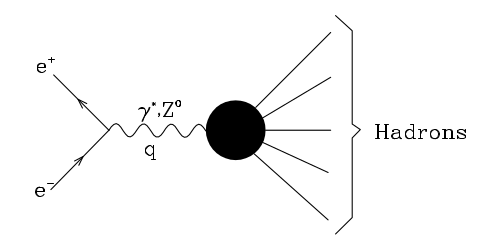
\includegraphics[width = 5 cm]{plots/ee_hadrons.png}
	\end{figure}	
	
	Consider corrections to $R_{0}$ from gluon radiation. Renormalize coupling.
	\begin{figure}
		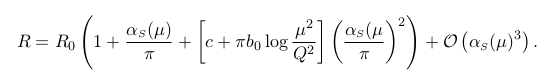
\includegraphics[width = 10 cm]{plots/eq_R0_3.png}
	\end{figure}

\end{frame}

% Hadron collisions III
\begin{frame}
	
	\frametitle{Hadron collisions}
	\framesubtitle{QCD from $e^{+}e^{-}$ annihilation}
	
	\begin{enumerate}
		\item Can we go to arbitrarily large energies? $\rightarrow$ divergences arise, renormalization / factorization needed
		\item Can we compute $R_{0}$ for every process? $\rightarrow$ IR observables
	\end{enumerate}	

\end{frame}

% Renormalization group I
\begin{frame}

	\frametitle{Hadron collisions}
	\framesubtitle{Renormalization group}
	
	\begin{enumerate}
		\item UV divergences are encountered in field theories
		\item Take a physical quantity $G$ depending on a scale $M$, a coupling $\alpha$ and some invariants $s_{1}, ..., s_{n}$	
		\item Define a "renormalized" $\alpha_{\textrm{Ren}} = \alpha + c_{1}\alpha^{2} + c_{2}\alpha^{3} + ...$
	\end{enumerate}
 
	The physical quantity in terms of $\{\alpha, M\}$ and $\{\alpha_{\textrm{Ren}}, \mu\}$ 
	\begin{figure}
		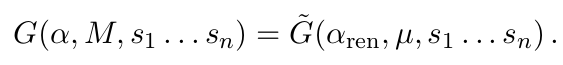
\includegraphics[width = 7 cm]{plots/eq_RGE.png}
	\end{figure}

	Physics must be invariant under change of $\{\alpha_{\textrm{Ren}}, \mu\}$
	\begin{figure}
		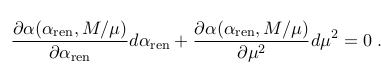
\includegraphics[width = 7 cm]{plots/eq_RGE_2.png}
	\end{figure}

\end{frame}

% Renormalization group II
\begin{frame}

	\frametitle{Hadron collisions}
	\framesubtitle{Renormalization group}
	
	\begin{itemize}
		\item Running coupling given by Renormalization Group Equation (RGE)
		\begin{equation}
		{\color{blue}\mu\frac{d\alpha_{s}(\mu)}{d\mu} = \beta(\alpha_{s}(\mu)) = -\sum_{n = 0}^{\infty} \beta_{n} \Big( \frac{\alpha_{s}}{\pi} \Big)^{n + 1}} \nonumber
		\end{equation}
		\item Coupling {\color{blue}$\alpha_{s}$} evolves with scale {\color{blue}$\mu$} as given by RGE $\rightarrow$ LO behavior driven by $\beta_{0}$
		\item $\beta_{0}^{\textrm{QCD}} < 0 \implies$ weakly coupled at large energies, asymptotic freedom
		\item $\beta_{0}^{\textrm{QED}} > 0 \implies$ strongly coupled at large energies, UV unsafe
		
	\end{itemize}

\end{frame}

% Jets in e+e- I
\begin{frame}
	
	\frametitle{Hadron collisions}
	\framesubtitle{Jets in $e^{+}e^{-}$}
	
	Consider $\alpha_{s}$ corrections to born level amplitude
	
	\begin{figure}
		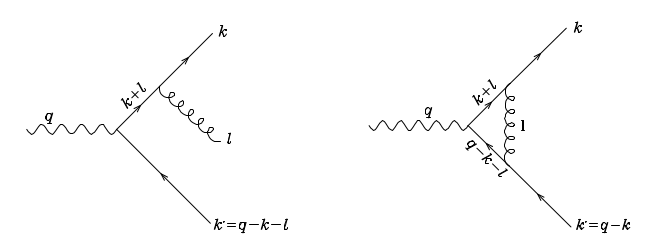
\includegraphics[width = 7 cm]{plots/qcd_corrections_2.png}
	\end{figure}

	\begin{align}
		\mathcal{M}_{\textrm{Born}} &= \bar{u}(k)\epsilon^{\mu}\gamma_{\mu}v(k') \nonumber \\
		\mathcal{M}_{1} &= \mathcal{M} \frac{k_{\alpha}}{k \cdot l} \nonumber \\
		\mathcal{M}_{1} &= -\mathcal{M} \frac{k'_{\alpha}}{k' \cdot l} \nonumber		 
	\end{align}

\end{frame}

% Jets in e+e- II
\begin{frame}

	\frametitle{Hadron collisions}
	\framesubtitle{Jets in $e^{+}e^{-}$}
	
	Consider $\alpha_{s}$ corrections to born level amplitude
	
	\begin{figure}
		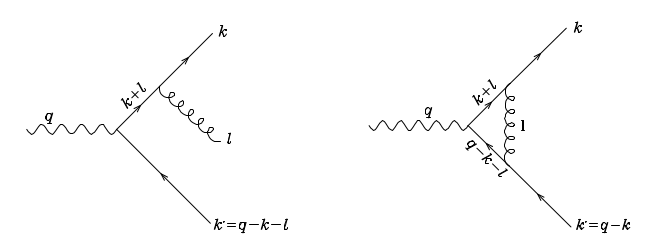
\includegraphics[width = 7 cm]{plots/qcd_corrections_2.png}
	\end{figure}
	
	Sum real and virtual contributions to the Born matrix element, with phase space element $d^{3}l = (l^{0})^{2} dl^{0} d\cos\theta d\phi$
	\begin{figure}
		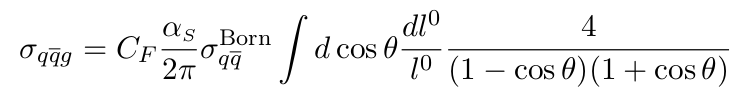
\includegraphics[width = 9 cm]{plots/eq_qqbg.png}
	\end{figure}

\end{frame}

% Jets in e+e- III
\begin{frame}

	\frametitle{Hadron collisions}
	\framesubtitle{Jets in $e^{+}e^{-}$}
	
	\begin{figure}
		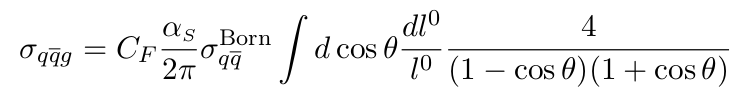
\includegraphics[width = 9 cm]{plots/eq_qqbg.png}
	\end{figure}

	\begin{itemize}
		\item Soft $(l^{0} \rightarrow 0)$ and collinear $(\theta \rightarrow 0, \pi)$ divergences
		\item No renormalization procedure to apply $\rightarrow$ divergences coming from long distance effects
		\item Kinoshita-Lee-Nauemberg theorem {\color{blue}(*)}
	\end{itemize}

\end{frame}

% Jets in e+e- IV
\begin{frame}

	\frametitle{Hadron collisions}
	\framesubtitle{Jets in $e^{+}e^{-}$}
	
	Sterman - Weinberg jets. "In a hadronic event with CM energy $E$, 2 cones can be found with opening $\delta$ containing $(1 - \epsilon)$ fraction of $E$."
	
	\begin{figure}
		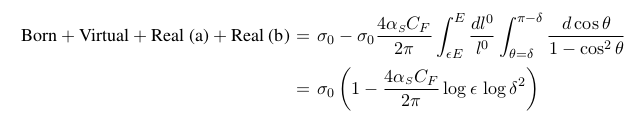
\includegraphics[width = 12 cm]{plots/eq_SW_jets.png}
	\end{figure}

	When all contributions summed, the cross section is no longer singular {\color{red}(*)}
	
\end{frame}

% Jets in e+e- V
\begin{frame}

	\frametitle{Hadron collisions}
	\framesubtitle{Jets in $e^{+}e^{-}$}
	
	Sterman - Weinberg jets. "In a hadronic event with CM energy $E$, 2 cones can be found with opening $\delta$ containing $(1 - \epsilon)$ fraction of $E$."
	
	\begin{figure}
		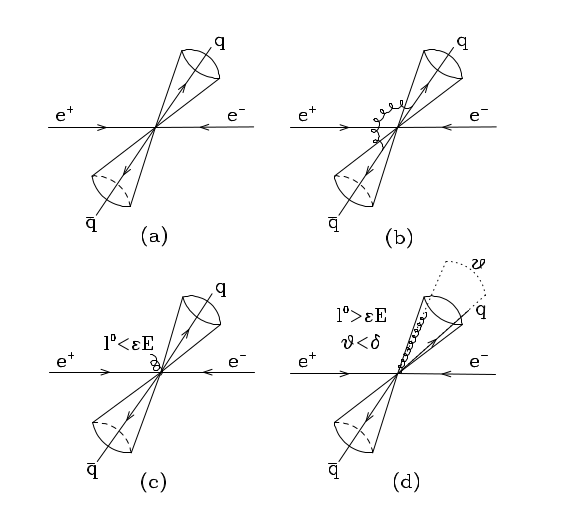
\includegraphics[width = 7 cm]{plots/SW_jets.png}
	\end{figure}

\end{frame}


% Collinear factorization
\begin{frame}

	\center{\color{blue}Collinear factorization}

\end{frame}

% Collinear factorization I
\begin{frame}

	\frametitle{Collinear factorization}
	\framesubtitle{QCD from $e^{+}e^{-}$ annihilation}
	
	\begin{itemize} 
		\item When computing partonic cross section, collinear partons can be emitted from incoming/outgoing parton.
		\item Cross section dominated by collinear decay
	\end{itemize}

	\begin{figure}
		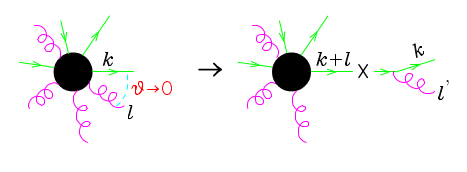
\includegraphics[width = 7 cm]{plots/collinear_factorization.png}
	\end{figure}

	Factorization theorem 
	\begin{figure}
	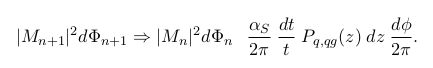
\includegraphics[width = 8 cm]{plots/eq_factorization_theorem.png}
	\end{figure}
	
\end{frame}

% Factorization theorem
\begin{frame}

	\frametitle{QCD in a nutshell}
	\framesubtitle{Factorization theorem}
	
	Observables in hadronic events $\longrightarrow$ $\sigma$ is hard to compute
	
	\begin{figure}
		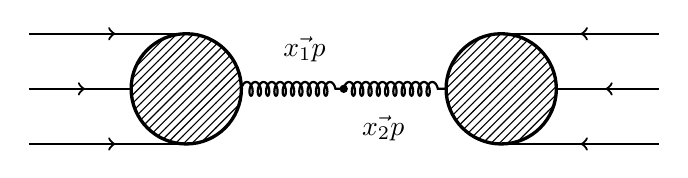
\begin{tikzpicture}
		% Incoming first proton 
		\draw [thick, fermion] (-4, 0.7)--(-2, 0.7);
		\draw [thick, fermion] (-4, 0)--(-2.7, 0);
		\draw [thick, fermion] (-4, -0.7)--(-2, -0.7);
		\draw [thick, very thick, pattern = north east lines] (-2, 0) circle [radius = 0.7];
		% Gluons
		\draw [thick, gluon] (-1.3, 0)--(0, 0);
		\draw [thick, gluon] (0, 0)--(1.3, 0);
		\node at (-0.5, 0.5) {$\vec{x_{1}p}$};
		\node at (0.5, -0.5) {$\vec{x_{2}p}$};
		\draw [thick, very thick, fill = black, pattern = north east lines] (0, 0) circle [radius = 0.03];
		% Incoming second proton
		\draw [thick, very thick, pattern = north east lines] (2, 0) circle [radius = 0.7];
		\draw [thick, fermionbar] (2, 0.7)--(4, 0.7);
		\draw [thick, fermionbar] (2.7, 0)--(4, 0);
		\draw [thick, fermionbar] (2, -0.7)--(4, -0.7);
		\end{tikzpicture}
	\end{figure}
	
	Factorize the problem $\longrightarrow$ Convolute the {\color{red}PDFs}  with the partonic ${\color{blue}\hat{\sigma}_{i j}}$
	
	\begin{equation}
		\sigma = \int_{0}^{1} dx_{1} \; dx_{2} \; {\color{red} f_{\alpha}(x_{1}, \mu_{F}) \ast f_{\beta}(x_{2}, \mu_{F})} \ast {\color{blue}\hat{\sigma}_{\alpha \beta}(\alpha_{s}(\mu_{R}), \mu_{F})} \; \nonumber
	\end{equation}
	
	\begin{itemize}
		\item Partonic {\color{blue}$\hat{\sigma}$} can be computed as perturbative series in $\alpha_{s}$
		\item {\color{red}PDFs} absorb the non perturbative effects, evaluated at $\mu_{F}$
	\end{itemize}

\end{frame}

% Dealing with divergences
\begin{frame}

\center{\color{blue}Dealing with divergences}

\end{frame}

% Partonic cross section and pQCD
\begin{frame}

	\frametitle{Partonic cross section and pQCD}
	\framesubtitle{Why do we need series expansion?}
	\begin{columns}
		
		\column{0.45\textwidth}
		
		\begin{enumerate}
			\item QCD in $e+e-$ collisions
			\item Measure only hadrons in the final state
			\item Factorization theorem helps us to understand short range interactions
		\end{enumerate}
		
		\column{0.45\textwidth}
		\begin{figure}[!htb]
			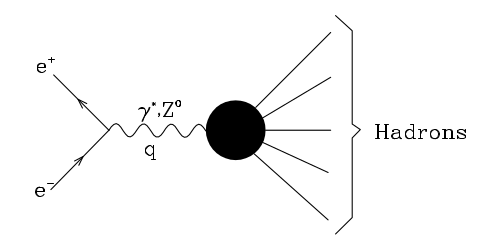
\includegraphics[width = \linewidth]{plots/ee_hadrons.png}
		\end{figure}
	
	\end{columns}
	
	\vspace{1cm}
	
	Write the cross section as a perturbative series
	\begin{equation}
		\hat{\sigma} = \sigma^{\texttt{Born}} \Bigg( 1 +
		\frac{\alpha_{s}}{2\pi} \sigma^{(1)} + 
		\Big(\frac{\alpha_{s}}{2\pi}\Big)^{2} \sigma^{(2)} + 
		\Big(\frac{\alpha_{s}}{2\pi}\Big)^{3} \sigma^{(3)} + ... \Bigg) \nonumber
	\end{equation}
	Leading order predictions can strongly depend on the renormalization and factorization scales $\rightarrow$ {\color{red}Go for higher order corrections!}
\end{frame}

% Perturbative QCD
\begin{frame}

	\frametitle{Perturbative QCD}
	\framesubtitle{Higher order corrections}
	\begin{columns}
	
	\column{0.45\textwidth}
	
	\begin{enumerate}
		\item Higher order corrections as virtual and real contributions
		\item Large number of diagrams to consider $\rightarrow$ harder to compute
	\end{enumerate}
	
	\column{0.45\textwidth}
	\begin{figure}[!htb]
		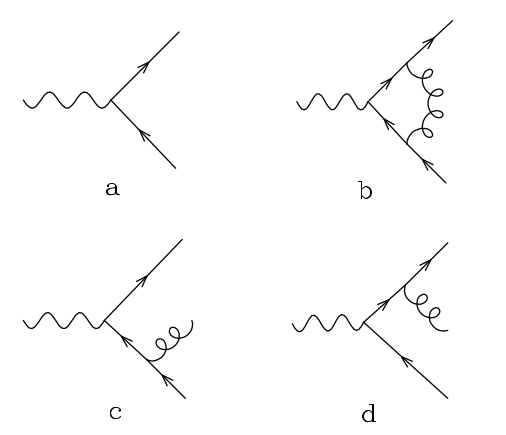
\includegraphics[width = \linewidth]{plots/qcd_corrections.png}
	\end{figure}
	
\end{columns}

\begin{equation}
	\sigma_{q\bar{q}g} = C_{F} \frac{\alpha_{s}}{2\pi} \sigma_{q\bar{q}^{\textrm{Born}}} \int d\cos\theta \frac{dl^{0}}{l} \frac{4}{(1 - cos\theta)(1 + cos\theta)} \nonumber
\end{equation}

	Fixed Order computations diverge!

\end{frame}

% Resummation QCD
\begin{frame}

	\frametitle{Resummation in QCD}
	\framesubtitle{Resumming large logs}

	Truncated fixed order predictions $\rightarrow$ divergent $\ln^{m}(M^{2}/q_{\perp}^{2})$ appear.\\
	Then the $q_{\perp}$ distribution need to be evaluated by replacing the partonic cross section as follows
	
	\begin{equation}
		\frac{d\hat{\sigma}_{ab}}{dq_{\perp}^{2}} \rightarrow 
		\Bigg[ \frac{d\hat{\sigma}^{\textrm{res.}}_{ab}}{dq_{\perp}^{2}} \Bigg]_{\textrm{l.a.}} + 
		\Bigg[ \frac{d\hat{\sigma}^{\textrm{fin.}}_{ab}}{dq_{\perp}^{2}} \Bigg]_{\textrm{f.o.}} \nonumber
	\end{equation}

	Resummed expression 
	\begin{equation}
		\frac{d\hat{\sigma}_{ab}^{\textrm{res.}}}{dq_{\perp}^{2}} = \frac{M^{2}}{\hat{s}} \int db \; \frac{b}{2} \; J_{0}(b q_{\perp}) \; \mathcal{W}_{ab}(b, M, \hat{s}; \alpha_{s}(\mu_{R}^{2}), \mu_{R}^{2}, \mu_{F}^{2}) \nonumber
	\end{equation}
	
	Being
	\begin{equation}
		\mathcal{W}_{N}(b, M, \hat{s}; \alpha_{s}(\mu_{R}^{2}), \mu_{R}^{2}, \mu_{F}^{2}) = \mathcal{H} \times exp\{\mathcal{G}\} \nonumber
	\end{equation}

\end{frame}

\begin{frame}

	\frametitle{Resummation in QCD}
	\framesubtitle{Resumming large logs}
		
		\begin{figure}[!htb]
			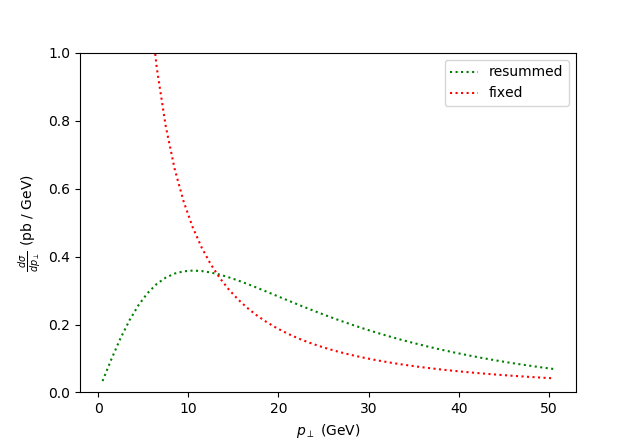
\includegraphics[width = 6 cm]{plots/hqt_resummed.png}
		\end{figure}
		
		\begin{enumerate}
			\item FO distribution diverges at small $q_{\perp}$
			\item Sudakov factor kills the divergence
			\item Matched at some intermediate accuracy
		\end{enumerate}

\end{frame}

% HTurbo
\begin{frame}

\center{\color{blue}HTurbo: Fast predictions for Higgs production}

\end{frame}

% HqT and HRes
\begin{frame}

	\frametitle{HqT and HRes}
	\framesubtitle{Predictions for Higgs $q_{\perp}$ distribution}
	
	\begin{figure}
		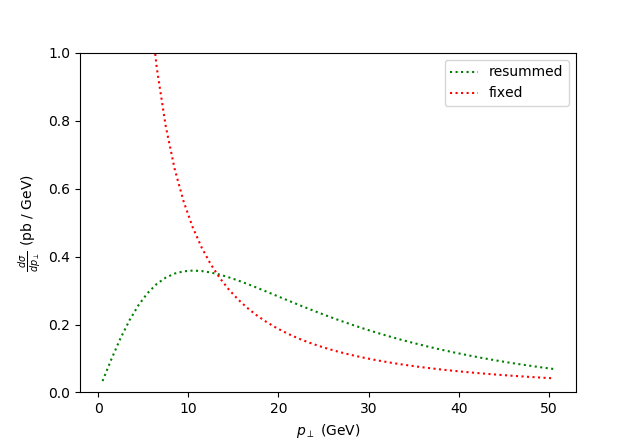
\includegraphics[width = 7 cm]{plots/hqt_resummed.png}
	\end{figure}
\end{frame}

% DYturbo
\begin{frame}

	\frametitle{HTurbo}
	\framesubtitle{Higgs distribution from Drell Yan}
	Take DYTurbo from \href{https://dyturbo.hepforge.org/}{DYTurbo}\\
	Ref. at \href{https://arxiv.org/abs/1910.07049}{1910.07049}
	\begin{enumerate}
		\item Matrix element
		\item Sudakov factors
		\item Hard coefficients 
		\item LO integration
	\end{enumerate}

\end{frame}

% Results
\begin{frame}

\frametitle{Results}
\framesubtitle{Comparison HTurbo and HqT}

\begin{figure}
	\minipage{0.32\textwidth}
	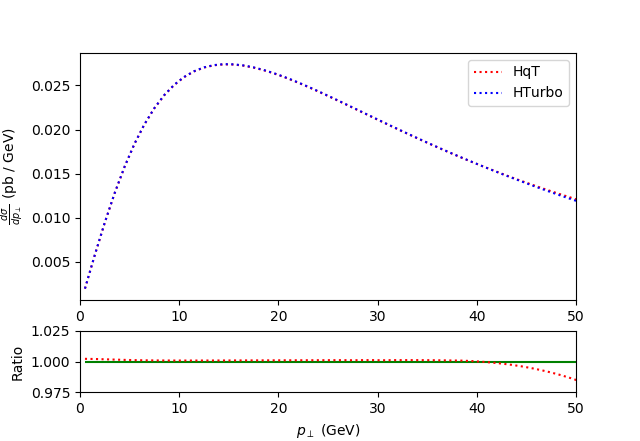
\includegraphics[width = \linewidth]{plots/hturbo_LL.png}
	\endminipage\hfill
	\minipage{0.32\textwidth}
	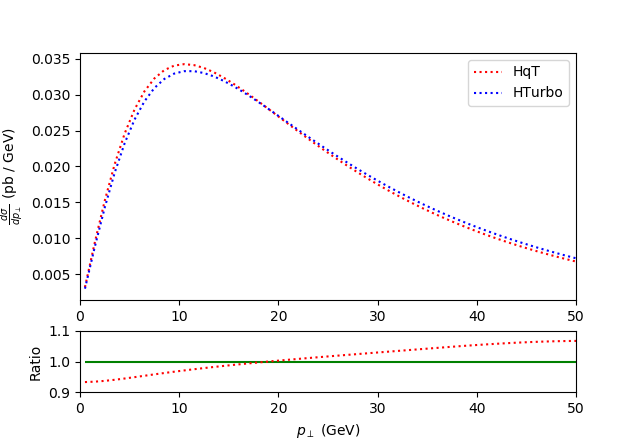
\includegraphics[width = \linewidth]{plots/hturbo_NLL.png}
	\endminipage\hfill
	\minipage{0.32\textwidth}
	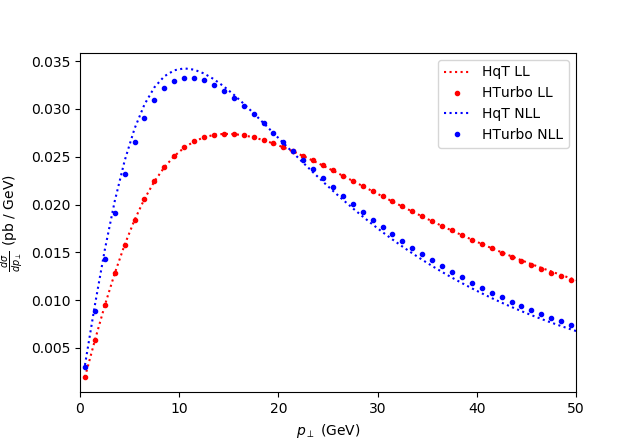
\includegraphics[width = \linewidth]{plots/hturbo_all.png}
	\endminipage
\end{figure}

\begin{itemize}
	\item HTurbo produces qt distributions that match HRes and HqT
	\item Excellent numerical agreement up to NNLO
\end{itemize}

\end{frame}

% Conclusions
\begin{frame}
	
	\frametitle{Summary $\&$ Conclusions}

	\vspace{2.0 cm}
	
	\begin{enumerate}
		\item Fast predictions are required towards the precision era of the LHC
		\item HTurbo produces qt distributions that perfectly match HRes and HqT
		\item Predictions by HTurbo are much faster than any of the existing codes
		\item Next steps: Implement PDF evolution N3LO distributions

	\end{enumerate}

	\vspace{2.0 cm}

	{\small \color{blue} This project has received funding from the European Union$'$s Horizon 2020 research and innovation program under grant agreement No 740006.}

\end{frame}

\end{document}